\chapter{Introduction}

\epigraph{Learning to read is probably the most difficult and revolutionary thing that happens to the human brain, and if you don't believe that, watch an illiterate adult try to do it.}{John Steinbeck}

\section{Overview}
Reading is a complex cognitive act. To read, individuals must precisely control visual attention, map symbols to sounds, extract meaning from words, maintain and update a mental model of the text events, inhibit unimportant associations, and make appropriate inferences. Consequently, reading difficulty can arise from many sources \citep{Pennington2009, vanderLely2010}. To further complicate matters, reading disability is often comorbid with other learning and developmental disorders, such as specific language impairment and attention deficit / hyperactivity disorder \citep{Pennington2006, Margari2013}.

Despite its complexities, the most explicit aim of reading instruction and intervention is to build fast and efficient orthographic-phonological mapping. This mapping process is a concrete skill that can be improved through practice, and which also serves as a bottleneck to the semantic processes: if an individual cannot decipher individual words, they will not be able to comprehend the meaning of blocks of text. However, while "phonics" instruction works better than other programs \citep{NationalReadingPanel2000}, critics can reasonably say that it is only part of a balanced educational program. But teasing apart the specific skills of that should be taught becomes much more difficult as they become less mechanical. For example, vocabulary size is often used as a proxy for the ability to comprehend speech, but this ignores important executive and attention skills \citep{Spencer2014}. Passage comprehension measures, on the other hand, are highly variable, both in their administration, skills assessed and resulting measures \citep{Cutting2009a}. 

Neuroimaging provides an alternative way of assessing what makes good readers successful, and it use has yielded valuable insights into the neural mechanisms of typical and atypical reading. Researchers have shown that reading co-opts the brain's visual system to introduce a new input pathway into existing language comprehension circuitry \citep{Jobard2007}. As text complexity increases, a larger demand is made on support systems, and activation becomes more bilateral and widespread \citep{Xu2005}.  Meta-analyses show that individuals with reading difficulty typically exhibit underactivation in areas responsible for recognizing symbol units, parsing acoustic sounds into phonological units, and binding letters to sounds \citep{Maisog2008, Richlan2009, Paulesu2014}. However, many questions remain regarding the root causes of dyslexia, how to best identify children at risk and the reasons for its high comorbidity with other developmental disorders. 

Connectivity-based neuroimaging methods provide an alternative framework to examine reading difficulties. Whereas traditional approaches focus on identifying focal regions of deficit, many learning and psychiatric disorders are characterized, in part, by how brain networks behave and interact. In particular, \textit{connectome} analyses have shown that the brain exhibits a network configuration which allows for high transferability of information at minimal cost, i.e. a “small-world” network architecture \citep{Bullmore2012}. Two attributes of brain organization have been of special interest: the presence of densely intra-connected \textit{modules}, often called resting-state networks (RSNs) \citep{Sporns2016}; and the existence of a core group of \textit{hub areas} that play an outsize role in conveying information between RSNs \citep{VandenHeuvel2011}. 

Since reading requires rapid interaction and manipulation of disparate cognitive processes, the network framework is an appealing avenue of investigation. Previous research has suggested that the areas responsible for reading do not form a single network, but are instead distributed across multiple RSNs \citep{Vogel2013}. There is evidence that the constitution of these RSNs (e.g. the default mode network) could be predictive of disorders, including attention deficits \citep{Uddin2008}. Furthermore, damage to hub areas can cause devastating behavioral effects \citep{Warren2014} and may be degenerated in psychiatric and developmental disorders such as schizophrenia, Alzheimer's disease and ADHD \citep{Stam2014}. Graph theory measures of connectedness within and between RSNs may consequently be related to differences in reading skill. However, while a small number of papers indicate that they may be affected in dyslexia \citep{Qi2016, Finn2014}, its application in the reading domain has been relatively sparse, with few emergent themes thus far \citep{Cao2016}. This is surpising because connectomics data can be procured without using cognitive tasks (which represent a confounding variable) and because they provide a common neurobiological framework for understanding cognitive disorders.

Taken together, the findings support a central thesis: it is not sufficient to describe reading comprehension solely as a set of independent processes. While understanding the reading-specific skills and their neural substrates is a necessary starting point, as seen in the literature on the visual word form area, a localization approach cannot account for changes in the interactions between systems of brain regions that may account for co-morbidity between developmental disorders and the influence of executive function on reading success. 

In this dissertation, I will flesh out a network description of the network-level processes important for reading comprehension. This chapter lays the theoretical groundwork: first, I describe metrics for measuring different aspects of network architecture and their potential significance to cognitive models. Then, I connect two principal aspects of a network persepctive - segregated RSNs and important hub areas - to reading processes and dyslexia. Finally, I discuss how maturation and education throughout development influence both reading skill and network architecture, and how the two might interact. I will then describe the three studies undertaken to establish the importance of a network approach to cognition.


\section{Methods for describing brain network architecture}

In 1995, Biswal et al. discovered that portions of motor cortex that were active during tasks were correlated when participants were not doing anything in particular, suggesting that there was an intrinsic relationship between these areas \citep{Biswal1995}. However, in the excitement of the early years of fMRI, these “resting-state” findings had little traction. In 2003, Greicius et al. found that the default mode network", a set of brain areas that was commonly seen anti-correlated during tasks, exhibited higher activity at rest \citep{Greicius2003}. Another paper from Yeo et al. identified a further six of these RSNs, and since then, scientists have been actively identifying and characterizing different RSNs that can be reliably found in individuals at rest \citep{Yeo2011}. A number of RSNs have been identified which may underlie cognitive function, including language \citep{Cordes2000, Hampson2002}, visual perception \citep{Simmons2012}, motor functioning \citep{Biswal1995} and executive control \citep{Seeley2007}. Although there can be significant variability between and even within scans \citep{Honey2009}, these functional connectivity findings are robust and have been repeatedly found in large scale datasets.

\begin{figure}[t]
    \centering
    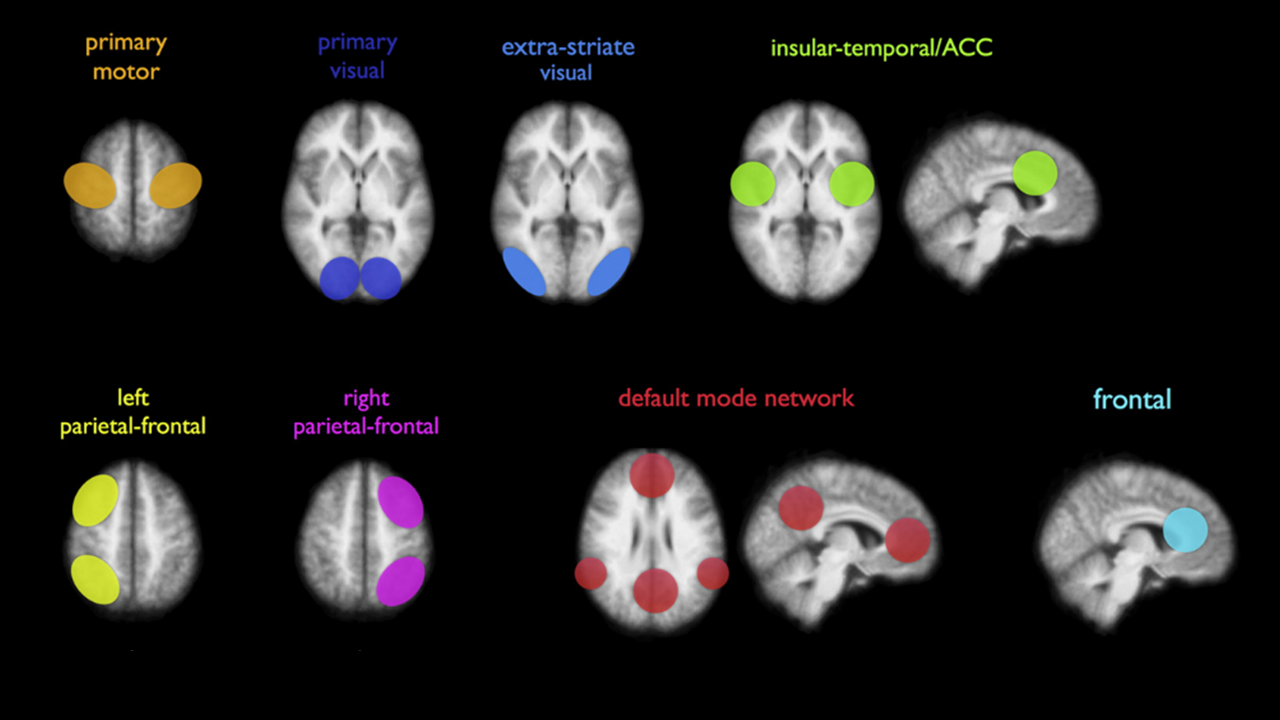
\includegraphics[height=3in]{images/ch1-ica.png}
    \caption[Examples of resting-state networks.]{Examples of resting-state networks derived from 16 adult subjects at rest. fMRI data were decomposed into 21 independent components and thresholded at p \textgreater 0.7.}
    \label{fig:ch1-ica}
\end{figure}

Beyond simply identifying these networks, scientists have used graph theory to analyze how the brain areas that make up these networks act in terms of the entire system of brain networks (sometimes called the connectome). In graph theory, each brain area is a single “node” in the larger brain network and temporal correlations with other nodes are “edges". In RS-fMRI, similar cortical areas (e.g. Brodmann areas) are typically assigned to to be nodes. In some cases, the entire brain is input into the analysis, whereas others use a more targeted, seed-based approach \citep{Vogel2010}.  Edges are often weighted, meaning areas that are more highly correlated carry a greater connectivity value. Next, an algorithm is applied to the matrix of correlations to distinguish sets of nodes that are more highly connected to each other than to other areas of the brain. Finally, first- and second-level properties of the networks, are derived.

The decision of which regions to include as nodes is critical. Typically, one of several approaches has been used to identify nodes: anatomical parcellations based on an atlas \citep{Supekar2008, Liu2008, Lynall2010}; individual voxels \citep{Fair2007}; functional ROIs from either a priori hypotheses or task-based activation \citep{VandenHeuvel2010}; or an algorithm that parcellates the brain independent of function or anatomy \citep{Goni2014}.  Differences in these methods can affect the RSNs identified. At high resolutions (e.g. voxel-level correlations), there is a greater chance of spurious correlations causing noise in the data; at lower resolutions, the timeseries for a region may blend multiple functional regions, creating a composite that does not truly reflect any of the underlying areas. 

Graph theory provides several metrics for consideration, of which we focus on three: \textit{modularity} is the number of connections a single node has \citep{Sporns2013}. Nodes with higher degrees are thought to communicate with a greater number of nodes than others; networks with a higher average degree are thought to be more densely connected.  The \textit{participation coefficient} is the degree to which a node participates in networks other than its primary one. Finally, \textit{path length} is the minimum number of nodes that must be passed to connect one node to any other. A completely random network will have a relatively low path length; a completely regular one will have a high path length. 

Developmentally, RSNs exhibit increasing functional correlation across the lifespan \citep{Kesler2013, Uddin2010}. Properties of these RSNs, including density of connections, along with their locations and changes with development is of primary interest  \citep{Cole2014, Dosenbach2007, Fair2009}. RSNs in children are more greatly constrained by proximity than in adults but are functionally organized: visual system regions, for example, form their own community, as do auditory regions and executive control regions \citep{Seeley2007}. Several studies report that the brain takes on a modular structure, consisting of many densely intra-connected networks \citep{Bullmore2009, Fair2009, Supekar2009, Dosenbach2007}. These modules are connected to each other by a smaller number of regions, dubbed “rich clubs” or “hubs", that may facilitate the passage of information from one module to another \citep{Power2013, Bullmore2012}.

\begin{figure}[t]
    \centering
    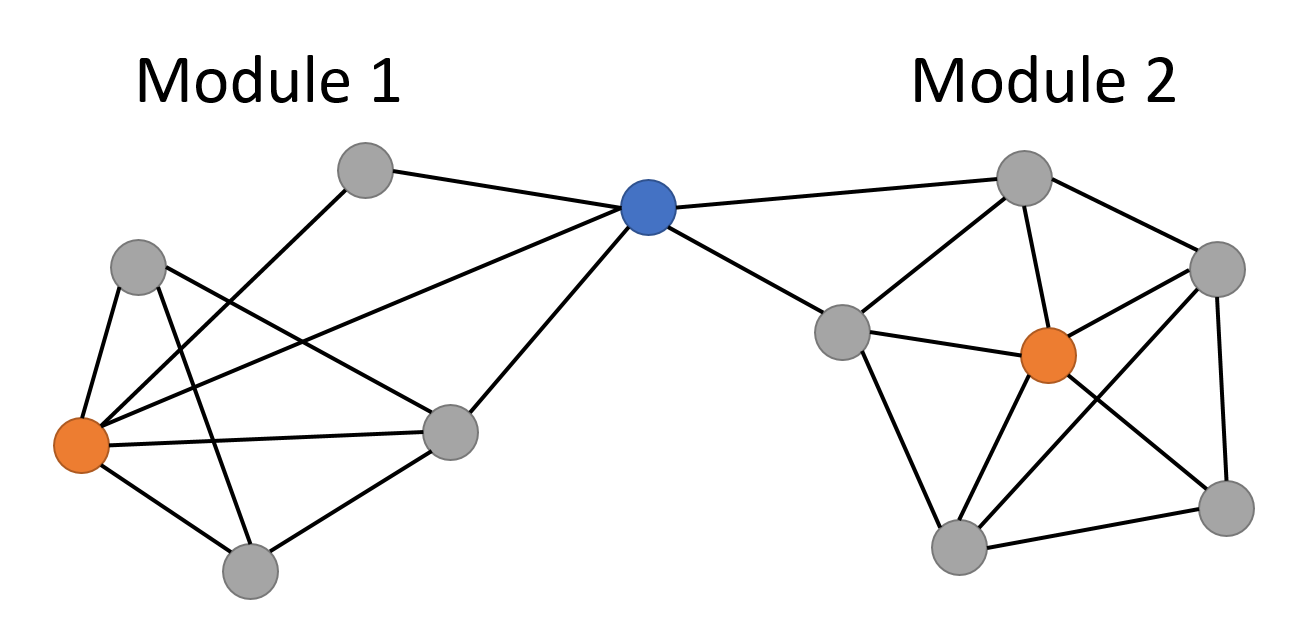
\includegraphics[height=3in]{images/ch1-graph-schema}
    \caption[Schematic for a network with two modules.]{Schematic for a network with two modules. The blue node is a hub region critical for connecting modules 1 and 2. The orange nodes have the highest degree of all nodes. Figure taken from \citep{Godwin2016}.}
    \label{fig:ch1-graph-schema}
\end{figure}

These findings have informed our understanding of the brain's large-scale organization. Rather than having a set of tracts that connect all regions, these findings suggest the brain is organized complexly but efficiently in a “small-world” architecture. This has emphasis on the importance of certain regions to fulfilling cognitive functions: in one study with lesioned patients, Petersen et al. predicted how severe a lesion would be based on its proximity to these hub regions \citep{Warren2014}. They found that lesions on areas that were not densely connected showed less extended impairments than regions which were highly inter-connected in RS-fMRI. Other psychiatric disorders have found disruptions in network properties. Lord et al. found that while whole-brain metrics of modularity were similar across individuals with depression and , RSNs “reorganized” in individuals with depression \citep{Lord2012}. Thus network properties may be important for explaining individual differences in neuropsychiatric disorders or cognitive skill, such as comprehension. 

However, the neurobiological basis for these RSN properties is still under investigation. While these connections do appear to be plastic and mediated by experience, they are not necessarily caused by new synapses. Several studies using diffusion-weighted MRI (DW-MRI) suggest that functional connectivity represents more than simply direct synaptic connections. Diffusion-weighted MRI (DWI) uses water movement to model the white matter tracts within the brain. At high resolutions, it provides a coarse approximation of the human connectome, i.e. the total connections in the human brain \citep{Sporns2005}. Honey et al. investigated whether functional connectivity can be predicted from structural connectivity \citep{Honey2009}. Five subjects underwent DW-MRI and RS-fMRI scans, and brains were parcellated at both a high resolution (998 cortical regions) and low resolution (66 cortical regions). They found that, while structurally connected areas are typically functionally connected as well, the inverse is not true. Areas that were closer together were also more highly functionally connected, possibly due to structural cortico-cortical projections. 

\section{The role of resting-state networks in reading}
While reading researchers in the past decade have begun to acknowledge the contributions of domain-general skills (e.g. attention, working memory, planning and organizing) to reading, it remains a secondary concern in much neuroimaging literature. (This is not the case for all language research but specifically reading.) To illustrate the widespread distribution of activity, Bailey et al. compared the meta-analytic activations maps from NeuroSynth with a popular resting-state network parcellation \citep{Bailey2018}. 

The results, shown in figure \ref{fig:ch1-yeo-to-neurosynth}, show that the visual and somatomotor-auditory RSNs consituted about one quarter of the NeuroSynth activations (17.5 and 8.2 percent, respectively), while attention networks combined to make up 37 percent. The fronto-parietal (19.3 percent) and default mode (17.8 percent) networks were were also highly represented. The limbic network was the only RSN which did not meaningfully overlap with the reading network. Compared to the baseline distribution of the Yeo parcellation, the visual, dorsal attention, ventral attention and fronto-parietal networks consituted a larger portion of the activation; the limbic, somatomotor and default mode had smaller shares. 

In the next few sections, we survey possible functions of these RSNs and hub areas might play during reading and in dyslexia.  

\begin{figure}[t]
\centering
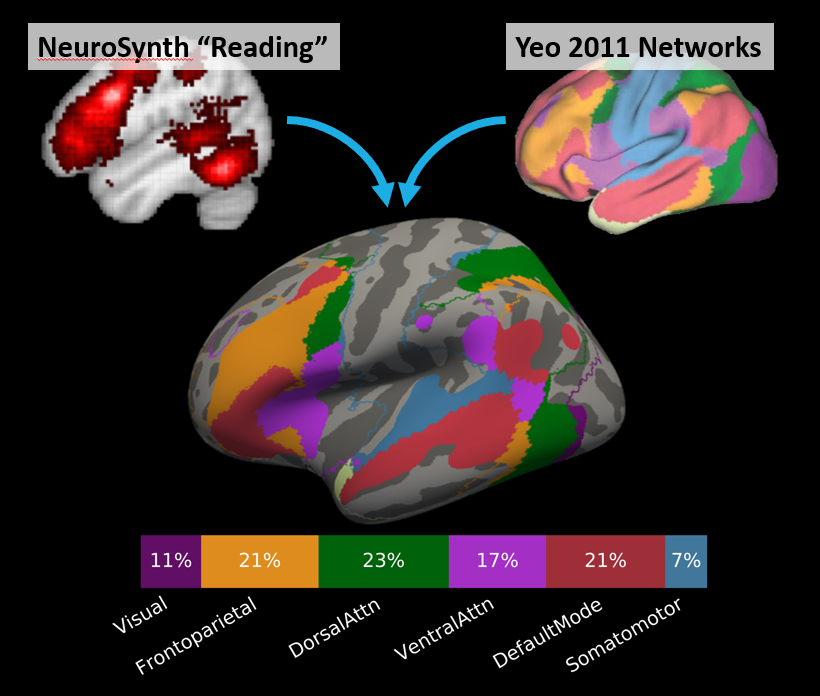
\includegraphics[height=3in]{images/ch1-yeo-to-neurosynth.png}
    \caption[Reading areas are distributed across many resting-state networks.]{Reading areas are distributed across many resting-state networks. On the left is the volumetric breakdown of the “reading” network, pulled from a NeuroSynth automated meta-analysis (forward-inference: $p < 0.01$, FDR-corrected) \citep{Yarkoni2011}, according to the 7-network cortical parcellation from Yeo and colleagues \citep{Yeo2011}. On the right is a surface plot of the same data. Reading areas are well-distributed across different networks and load highly onto attention and executive networks. Several important reading areas, including the inferior frontal gyrus and temporo-parietal junction, sit at points where multiple networks converge, i.e. likely hub areas.}
    \label{fig:ch1-yeo-to-neurosynth}
\end{figure}

\subsection{The visual word form area is part of the DAN} 
The visual word form area (VWFA) performs an important role in orthographic processing, and activity in the VWFA is sensitive to letter size, font and other orthographic attributes \citep{References from Vogel2011}. It's alleged specificity to language has been a source of controversy over the past decade \citep{McCandliss2003a}, however, and several have argued that its importance in reading is directly linked to its membership in the DAN \citep{Vogel2012a}. During reading, the DAN supports appropriate textual features or chunks and suppressing distracting information elsewhere \citep{Corbetta2002}. At issue in the debate is how general or specific visual attention deficits are in dyslexia \citep{Vogel2014}. Decreased activation in the pVWFA to text relative to typically developing participants has been reported in several studies of dyslexia \citep{Richlan2009}, but these differences could be due to more generalizable visuo-spatial deficits. For example, fluent reading requires accurate and precise eye movements \citep{Rayner1998}, and a key node in the DAN is the “frontal eye fields” which help coordinate saccadic activity \citep{Petit1997,Connolly2000}. In fact, a number of studies report deficits in visual attention in children with RD \citep{Vidyasagar2010}. Children with RD deficits in processing of consonant strings \citep{Pammer2004} and in matching symbol strings \citep{LassusSangosse2008}. Koyama et al.  found that children with a historical diagnosis of dyslexia had persistant de-coupling of the dorsal attention network compared to typical readers regardless of remediation status \citep{Koyama2013}. Vogel et al.  found that reading ability in typical children and adults (including decoding and passage comprehension ability) predicted increased correlations between the visual word form area and the dorsal attention network \citep{Vogel2012a}. Whatever the true cause, it is clear that the DAN provides critical support for reading, above and beyond simply processing stimuli.

\subsection{Attention networks drive and suppress sensory integration} 
Attention underlies skilled reading at all levels: it is critical for identifying only the salient words in a large block of text, for suppressing environmental distractions and for maintaining focus for extended periods of time. In a common framework for attention, the dorsal and ventral attention networks (DAN and VAN) play collaborative roles for guiding focus. (The “salience” network, is sometimes differentiated from the VAN.) Simplistically, the DAN exerts top-down control of sensory processes to keep a person on task, while the VAN detects salient or unexpected stimuli, acting as a “circuit breaker” to help reorient the person \citep{Corbetta2002, Vossel2014}. This relationship may be impaired in individuals with dyslexia that have “sluggish attention shifting” attention between visual and auditory modality \citep{Harrar2014}. Slow or inadequately rapid attention-shifting could undermine fluent reading by causing temporal-spatial misalignment in processing, e.g. letter sequence and arrangement \citep{Lallier2009}. This deficit in attentional shifting is argued to further characterize dyslexic readers’ rapid temporal and low spatial frequency processing \citep{Witton1998}, and asynchronicity within this system is argued to be characteristic of dyslexia \citep{Lallier2009}. Online interaction between the DAN and VAN during reading may thus index some of the attentional switching problems that are apparent in dyslexia. 

\subsection{Executive networks coordinate other cognitive processes} 
Executive functions play an important role in predicting reading outcomes, especially when considering comprehension \citep{Cutting2009a}. Although the variety of cognitive processes that fall under EF construct do not map cleanly onto a single brain region or network, they are closely associated to the “central executive” system. This in turn is mapped on to the fronto-parietal network (FPN) (and sometimes the cingulo-opercular network) \citep{Fedorenko2014a, Cocchi2013}. Unlike many other RSNs, the FPN has components which are not neighboring, spanning portions of the frontal and parietal lobes \citep{Yeo2011}. Interestingly, the FPN has recently been hypothesized to act as a neural mediator of other brain systems \citep{Mennon2010, Cole2014} by using wide-spread cortical connections to facilitate efficient processing of other networks, and in particular assist when areas are not functioning adequately. According to this coordinator model of the FPN, greater symptoms of dyslexia may correspond with reduced functional and structural integrity of the FPN. For instance, Norton et al. compared brain activation and connectivity in DYS reader sub-types, including readers with rapid naming deficits only, phonological awareness deficits only, and double deficits (i.e. poor rapid naming and phonological awareness) \citep{Norton2014}. They found graded de-activation and de-coupling of the FPN during a word rhyme judgment task, with the most severe deficit sub-group (double deficit) showing the greatest FPN de-activations and internal de-coupling. In the only functional connectomics paper on young readers with dyslexia, Finn et al. (2013) examined whole-brain connectivity during a word/non-word rhyming task, and found that children (and adults) with dyslexia showed de-coupling of frontoparietal areas \citep{Finn2014}. 

\subsection{Executive networks may support intervention response}
In addition to coordinating other RSNs, the FPN may play a role in supporting systems \citep{Cole2014}. Horowtiz-Kraus et al. (2015) examined resting state functional connectivity in young readers with and without dyslexia who had undergone a reading intervention \citep{HorowitzKraus2015}. They found that after intervention, readers with dyslexia had improved connectivity between a visual component and bilateral regions in the FPN (notably, as in many studies on reading, the latter component was not identified as an FPN component, but instead discussed as a language network). Furthermore, Koyama et al. (2013) examined resting state connectivity in dyslexic readers with variable remediation status, and found that children with a historical diagnosis of dyslexia had persistent de-coupling of frontoparietal areas compared to typical readers, regardless of remediation status \citep{Koyama2013}. Additionally, in the first reading study to examine functional interactions across networks, Aboud et al. (under review) found that, prior to intervention, readers who were responsive to the intervention mediated reading network connectivity via a key node in the FPN, the dorsolateral prefrontal cortex (dlPFC) \citep{Aboud2018}. These findings support the hypothesis that executive areas in the FPN might act to facilitate the functional integrity of other systems necessary for reading.

\subsection{Default mode network engagement and disengagement} 
The DMN is a network of inter-connected regions (including medial prefrontal cortex, bilateral inferior parietal lobules, and posterior cingulate cortex) \citep{Raichle2001}. Since its original discovery, the DMN has since been found to support a wide range of cognitive processes often classified under internal mentation \citep{Buckner2008}, including theory of mind, narrative processing, and autobiographical recall \citep{AbdulSabur2014}. The DMN exhibits a large amount of overlap with traditional reading areas, including major comprehension-related regions such as the angular gyrus and anterior temporal pole. However, the DMN also has antagonistic relationship with “task-positive” attention networks such as the FPN, where the activation of one network necessarily comes at the suppression of the other, and this relationship appears to be important for performance on a variety of cognitive processes \citep{Fox2005, Keller2015}. Consequently, appropriate FPN involvement may be best achieved by suppression of the DMN. Several studies point to over-involvement of the DMN in readers with dyslexia, including higher internal correlations of the DMN during reading \citep{Finn2014} and greater correlations between the DMN and reading areas during reading and at rest \citep{Schurz2014}. Given that activity in both the FPN and DMN are critical for reading comprehension, understanding the dynamics of this relationship could be particularly illuminating.

\subsection{Hub areas show abnnormalities in dyslexia}
Two decades of neuroimaging research have allowed a relative consensus to form as to which brain regions are commonly dysfunctional in dyslexia. To determine whether there was any pattern related to network architecture in these areas, we gathered all clusters from three meta-analyses comparing fMRI activation for individuals with dyslexia to typical readers \citep{Maisog2008, Richlan2009, Paulesu2014}. All areas that showed atypical activation in dyslexia (either greater or less activity) were included. When a cluster was large, all reported local maxima were included. 

\begin{figure}[t]
\centering
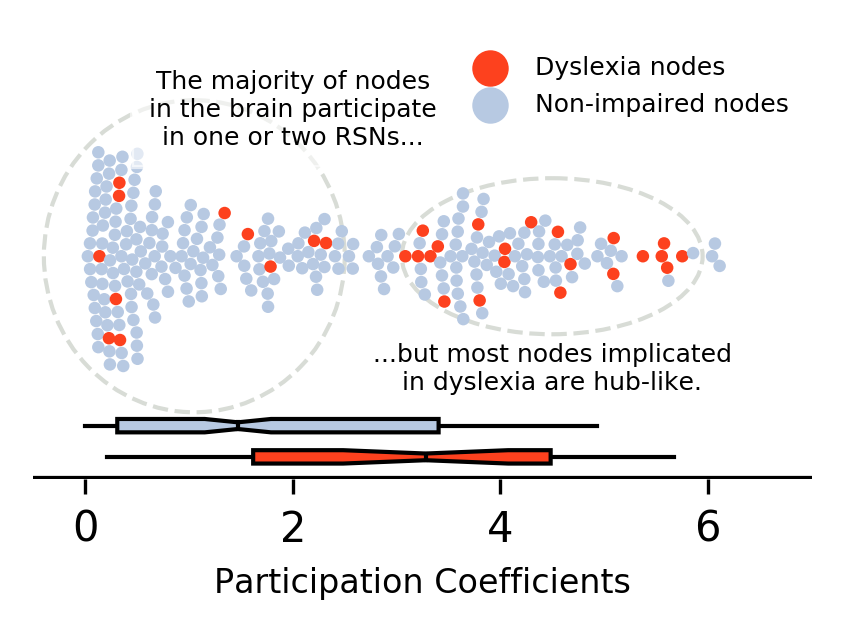
\includegraphics[height=3in]{images/ch1-dyslexia-hubs.png}
    \caption[Dyslexia disproportionately impacts hub areas.]{Dyslexia disproportionately impacts hub areas. Among the brain areas examined in Power and colleagues (2013), nodes implicated in dyslexia have higher participation coefficients (32 nodes) compared to the rest of the brain (232 nodes).}
\label{fig:ch1-dyslexia-hubs}
\end{figure}

To get measures of hubness across the brain, we used data from a connectomics study \citep{Power2013}. That study reports the \textit{participation coefficient} for each of the 264 nodes previously described. The participation coefficient reflects the diversity of a node's connectivity to different RSNs, where a higher value indicates that the node is correlated with many different RSNs. Activations from the dyslexia meta-analyses were then mapped to the geometrically closest node from this dataset, resulting in a small set of dyslexia-related nodes and a larger, unaffected set.

The distribution of participation coefficients across the 264 nodes was non-normal, with a large group of areas having low participation coefficients (i.e. affiliated with few RSNs) and a smaller hub-like group. Therefore, a Wilcoxon rank-sum test was performed on the participation coefficients for the two groups, which tests for the equivalence of two distributions in a non-parametric fashion.

Across the three meta-analyses, 32 of the 264 nodes showed abnormal functioning in dyslexia. Figure 3 shows the node-by-node distribution of participation coefficients for the entire set. The median participation coefficient for unaffected nodes was 1.47; for dyslexia-related nodes it was 3.28. A Wilcoxon rank-sum test between the dyslexia and unaffected nodes showed that dyslexia affects brain areas with higher participation coefficients than would otherwise be expected ($U = 4946.0$, $p$ \textless $0.001$). 


\section{Influence of development on network connectivity}

Children are taught to decode words between the ages of four and nine. This is a time of major developmental changes in the brain, with extensive synaptic pruning and myelination of white matter tracts \citep{Wandell2013}. The brain areas responsible for fast and efficient word decoding may become specialized through a process of \textit{interactive specialization}, in which intrinsic developmental processes and experience collaborate to form the mature, skilled reading system \citep{Johnson2011, Klingberg2014}. The theory is an extension of the Hebbian maxim that “neurons that fire together, wire together", with the brain being considerably more plastic during this developmental period than it is later in life \citep{Hebb1949}.

\begin{figure}[h!]
\centering
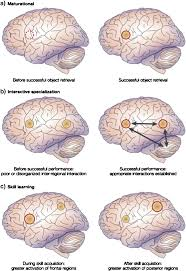
\includegraphics[height=3in]{images/ch1-interactive-specialization.jpg}
    \caption[Interactive specialization explains changes in activity.]{Interactive specialization posits that repeated co-activation of distant brain areas will create a network of regions important for performance of a given task. Figure taken from \citep{Gaffrey2013}.}
\label{fig:ch1-interactive-specialization}
\end{figure}

This process of interactive specialization may cause lasting changes to connectivity even when subjects are not reading. Evidence for this comes from resting-state fMRI, which does not require individuals to complete tasks but instead uses spontaneous neural activity from the fMRI signal to construct networks. Koyama et al. found that many reading-related nodes had overlapping connectivity with the left inferior frontal gyrus and left middle temporal gyrus, both nodes that are important for skilled language use \citep{Koyama2010}. A follow-up study comparing IQ-matched children and adults found similar patterns: better readers in both groups showed increased connectivity between the inferior frontal gyrus and the middle and superior temporal gyri, as well as between the precentral gyrus and motor areas \citep{Koyama2011}. In adults, positive correlations were found between reading ability and connectivity between the visual word form area and phonological processing areas; in children, however, this correlation was weaker and negative, suggesting that the visual word form area becomes more integrated with experience as well as skill. Reading intervention also exerts an effect on connectivity patterns. Dyslexic adolescents who received reading remediation had higher correlations between the visual word form area and the right middle occipital gyrus than did control participants \citep{Koyama2013}. This connectivity also correlated with spelling and single-word reading scores.

However, word recognition skill is insufficient to explain individual differences in comprehension \citep{Gough1986, Hoover1990}. That is, comprehension requires more areas of the brain than do those of more basic reading skills. Multiple studies have shown that in single-word reading tasks, neural activity is largely confined to areas near the visual system in fusiform regions, whereas in sentence and passage comprehension, readers utilize a broader array of brain regions \citep{Rimrodt2009, Xu2005}. Other reports corroborate these larger activations: Cutting et al. used a sentence comprehension task which elicited bilateral temporal lobe activation (left \textgreater right) and greater occipital lobe signal, as would be expected from increased language and visual load. Thus, sentence comprehension relies on a core set of extended language regions above that required for words.  \citep{Cutting2006a}. Consistent with theory, as readers become more skilled, patterns become more focused and sharply defined; in contrast, those who continue to struggle with reading (i.e. dyslexia) continue to show a more diffuse pattern of activity \citep{Rimrodt2009}. 

Relatively few studies have been done relating network methods to reading ability. Despite the changes in connectivity between areas, reading-related regions such as the fusiform gyrus, angular gyrus and inferior frontal gyrus, do not create one distinct RSN, but are members of separate, more primary RSNs \citep{Vogel2013}. Finn et al. compared graph theory metrics of dyslexic and non-impaired readers using graph metrics \citep{Finn2014}. Dyslexic readers showed divergent activity in visual association and prefrontal attention areas as well as increased right-hemisphere connectivity. Differences were persistent across both adult and children readers, suggesting that network metrics are relevant for reading. Another study investigating how graph theory metrics changed in response to sentence-level processing showed that network properties were relatively stable \citep{Ye2012}. Participants were asked to silently read a sentence that had either a semantically congruent or incongruent ending. Furthermore, metrics showed that subcortical processing (basal ganglia to supplementary motor area) was stronger in response to incongruent versus congruent endings. 

According to the view of interactive specialization, an integrative ability like reading comprehension would be more highly connected. The multi-RSN robustness, or the how well-maintained the network is after deletion of a node, will measure how strongly inter-connected the RSNs of interest are to each other \citep{Bullmore2009}. An important consequence of these hypotheses is that, if there is a biological substrate underlying RC, we may have another window into predicting how well a child will continue to develop as a reader, especially during the periods of rapid development in primary school.


\section{Conclusions}


We have establisehd that the network model for reading has particular bearing in models of reading, and that graph theory methods provide a summary framework with which to investigate the interactions between processes. Furthermore, development of cognitive skills is facilitated by the interactions between regions, rather than solely by themselves - but the study of these processes have not been investigated extensively. 

In this dissertation, I present three studies that investigate network properties as they relate to reading comprehension and reading success. The common thread is that reading requires the integration of many different brain networks (even moreso than listening) and that better readers are more able to meet these demands, even from a young age.

\begin{itemize}
    \item \textit{Study 1} investigates differences in global network topology between reading and listening and then hones in on changes to executive and attention networks 
    \item \textit{Study 2} looks at changes to whole-brain connectivity patterns in reading comprehension throughout development using a cohort of subjects aged 8 to 28
    \item \textit{Study 3} investigates individual differences in reading skill and its relationship to “intrinsic” network topology, using a large resting-state fMRI dataset with subjects spanning the many stages of development
\end{itemize}

Throughout, I will be leveraging fMRI and behavioral data collected in the Education and Brain Sciences Research Laboratory at Vanderbilt University. 

